\documentclass{../qh_exercise}
\graphicspath{ {./images/} }

\begin{document}

\section{Leerdoelen}
\begin{itemize}
	\item \texttt{x,y} co\"ordinaten om kunnen zetten in de \texttt{PVector} objecten.
	\item Gebruik kunnen maken van de volgende PVector methods: \texttt{add(PVector p), sub(PVector p), mult(float amount), rotate(float angle)}
\end{itemize}

\section{Uitleg}
\begin{itemize}
\item\myhref{https://natureofcode.com/book/chapter-1-vectors/}{Nature Of Code Chapter 1}\\Alleen \textbf{1.1, 1.2, 1.3, 1.4, 1.5}
\item\myhref{https://www.youtube.com/watch?v=mWJkvxQXIa8\&list=PLRqwX-V7Uu6ZwSmtE13iJBcoI-r4y7iEc}{Vectors - The Nature of Code}\\Alleen \textbf{1.1, 1.2, 1.3, 1.4}
\end{itemize}

\section{Voorbeelden}
\begin{enumerate}
	\item \texttt{star}
	\item \texttt{square}
	\item \texttt{forest}
	\item \texttt{flower}
\end{enumerate}

\newpage
\section{Opdrachten}
Omdat het onhandig is om telkens twee argumenten mee te moeten geven voor een positie op het scherm \texttt{int x, int y} en we een betere manier nodig hebben om met co\"ordinaten om te gaan bestaat er in Processing de \texttt{PVector} class.

\subsection{[optioneel] Vectoren in de wiskunde}
Een vector is een verzameling van meerdere variabelen. Wij zullen ons alleen maar bezig houden met 2 dimensionale vectoren van \texttt{x,y} co\"ordinaten.
Een vector wordt als volgt genoteerd: 
$$
\vec{v}=
\begin{pmatrix}
2\\3
\end{pmatrix}
$$
Er zijn een paar rekenregels, die erg voor de hand liggen als je bedenkt dat een vector gewoon een verzameling van twee co\"ordinaten is:
$$
\begin{pmatrix}
a\\b
\end{pmatrix}
+
\begin{pmatrix}
c\\d
\end{pmatrix}
=
\begin{pmatrix}
a + c\\b + d
\end{pmatrix}
$$

$$
a * 
\begin{pmatrix}
b \\ c
\end{pmatrix}
=
\begin{pmatrix}
a*b\\a*c
\end{pmatrix}
$$
De tweede rekenregel heet \textit{scalaire vermenigvuldiging}. Dit geeft het uitrekken of inkrimpen van een vector weer. Dit is makkelijker te zien als we de vectoren als pijltjes (of natuurkundige krachten) tekenen:\\
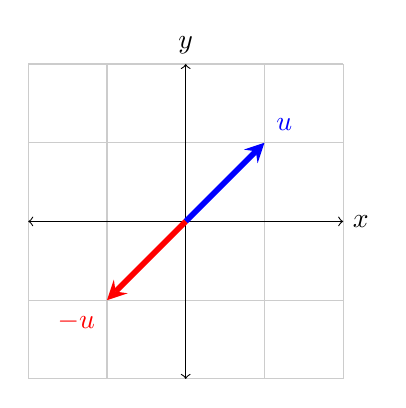
\begin{tikzpicture}
  \draw[thin,gray!40] (-2,-2) grid (2,2);
  \draw[<->] (-2,0)--(2,0) node[right]{$x$};
  \draw[<->] (0,-2)--(0,2) node[above]{$y$};
  \draw[line width=2pt,blue,-stealth](0,0)--(1,1) node[anchor=south west]{$\boldsymbol{u}$};
  \draw[line width=2pt,red,-stealth](0,0)--(-1,-1) node[anchor=north east]{$\boldsymbol{-u}$};
\end{tikzpicture}
\subsubsection{Opdrachten}
\begin{enumerate}
	\item Teken de optelling van $\begin{pmatrix}2\\1\end{pmatrix}+\begin{pmatrix}-1\\3\end{pmatrix}$
	\item Bereken $2*((3*\vec{a})+\vec{b})$ met $\vec{a}=\begin{pmatrix}1\\2\end{pmatrix}$ en $\vec{b} = \begin{pmatrix}-1\\2\end{pmatrix}$
	\item Bepaal het midden tussen $\vec{a}$ en $\vec{b}$. (We zoeken dus een algemene formule voor het midden tussen twee vectoren).
	\item Bereken de vector op $\frac{2}{3}$ afstand tussen $\vec{a}$ en $\vec{b}$ (Wederom zoeken we dus een algemene formule).
\end{enumerate}

\subsection{[Optioneel] PVector}
Processing heeft de class \texttt{PVector}, met daarin een heleboel handige methods, zie \texttt{https://processing.org/reference/PVector.html}
\begin{lstlisting}
	void setup() {
		PVector v1 = new PVector(3,2);
		PVector v2 = v1.copy();
		v1.add(v2);
		v2.sub(new PVector(1,1));
		v1.mult(3);
		drawDot(v1);
		drawDot(v2);
	}
	
	void drawDot(PVector v) {
		circle(v.x,v.y,5);
	}
\end{lstlisting}
\remark{De oorsprong (0,0) zit bij computers links boven, en niet links onder zoals bij de meeste wiskundige grafieken! De y-as is als het ware gespiegeld!}
Op welke co\"ordinaten tekent dit stukje code een stip?
Schrijf je antwoord in een \textit{comment} van je sketch:

\subsection{[Optioneel] Vectoren gebruiken}
Nu je hebt geleerd wat een vector is wil je natuurlijk deze coole vectoren voor alles gebruiken! Helaas accepteren de Processing functies geen vectoren, alleen \texttt{x, y} co\"ordinaten. Maak de volgende 3 functies af, de functie \texttt{myLine} is al gegeven.
\begin{lstlisting}
void myLine(PVector v1, PVector v2) {
    line(v1.x,v1.y,v2.x,v2.y);
}

void myCircle(PVector v1, int r) {
    // TODO
}

void myTriangle(PVector v1, PVector v2, PVector v3) {
    // TODO
}
\end{lstlisting}

\subsection{Een driehoek}
Maak de functie
\begin{lstlisting}
void betterTriangle(PVector p1, PVector side) {
    // TODO
}
\end{lstlisting}
Hierbij is \texttt{p1} \'e\'en van de hoekpunten en \texttt{side} \'e\'en van de zijden.
\tip{Kijk naar voorbeeld \texttt{square}}
\begin{figure}[H]
	\centering
	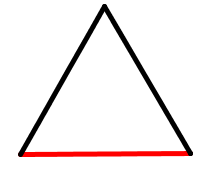
\includegraphics[width=\textwidth/4]{triangle.png}
	\caption{Een triangle met de vector \texttt{side} rood gekleurd}
	\label{fig:triangle}
\end{figure}

\subsection{Polygoon}
Een gelijkzijdige polygoon of veelhoek is een figuur met \texttt{n} hoeken en lijnstukken van gelijke lengte. Voor \texttt{n = 3} is dit een \textit{driehoek}, voor \texttt{n = 4} is dit een \textit{vierkant}, voor \texttt{n = 5} is dit een \textit{pentagon} en voor \texttt{n = 17} is dit een \textit{heptadecagoon}. Maak de volgende functie:
\begin{lstlisting}
	void polygon(PVector center, int radius, int n) {
	}
\end{lstlisting}
Deze functie moet een polygoon van \texttt{int n} hoeken tekenen met een straal van \texttt{int radius}. Maak gebruik van vectoren en gebruik de \texttt{rotate(float angle)} method. \\
\remark{Een hoek wordt niet in graden uitgedrukt maar in radialen, dit betekent dat \'e\'en cirkel (dus 360 graden) gelijk is aan $2 * \pi$, ofwel: \texttt{2 * PI}.}
\begin{figure}[h!]
	\centering
	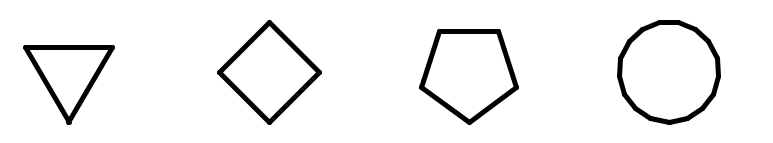
\includegraphics[width=\textwidth]{polygon.png}
	\caption{Polygonen met n = 3, 4, 5 en 17}
	\label{fig:polygon}
\end{figure}


\subsection{Middelloodlijn}
Maak de volgende functie aan:
\begin{lstlisting}
	void bisector(PVector p1, PVector p2) {
	}
\end{lstlisting}
Deze functie moet de middelloodlijn tekenen van de twee functies met de lengte gelijk aan de afstand tussen de twee functies (zie figuur \ref{fig:bisector}). \tip{Probeer eerst op papier een aantal middelloodlijnen te tekenen en probeer vervolgens om de twee punten waartussen de lijn getrokken moet worden te vinden.}
\begin{figure}[H]
	\centering
	
\includegraphics[width=4cm]{bisector.png}
	\caption{Middelloodlijn, de twee stippen geven \texttt{p1} en \texttt{p2} aan}
	\label{fig:bisector}
\end{figure}

\end{document}